\documentclass{article}
\usepackage{graphicx}
\usepackage{lmodern}  % for bold teletype font
\usepackage{amsmath}  % for \hookrightarrow
\usepackage{xcolor}   % for \textcolor
\usepackage{listings}
\lstset{
  basicstyle=\ttfamily,
  columns=fullflexible,
  frame=single,
  breaklines=true,
  postbreak=\mbox{\textcolor{red}{$\hookrightarrow$}\space},
}
%Enumering lower case roman numerals
%\renewcommand{\theenumi}{\roman{enumi}}   
%\renewcommand{\labelenumi}{\theenumi)}


\begin{document}

\title{\vspace{-2.0cm}Drone Precision Landing\\IDP 2022}

\author{Neil Dhami \\EE18BTECH11031	}

\maketitle
%-------------------------------------------------------------------------------
Download all python codes from 
\begin{lstlisting}
https://github.com/neildhami18/IITH_Academics/DroneIDP-2022/Manual-3/codes
\end{lstlisting}

%
and latex-tikz codes from 
%
\begin{lstlisting}
https://github.com/neildhami18/IITH_Academics/DroneIDP-2022/Manual-3/
\end{lstlisting}

\section{Introduction}
Conventional GPS on drones are only accurate to around 10 feet. Precision Landing refers to any landing methodology which is accurate to around 10 inches. For many drone applications, such as, Package delivery, Precision Agriculture, and Surveillance, the ability to land on a target is crucial. This manual describes a precision landing experiment using RPi camera module, empowered with OpenCV for tracking an image (Aruco Marker) on the ground. The range of this method is a function of the ground target image size and the resolution of frames in OpenCV script. Any altitude should work given a high enough resolution and the right sized marker is used


\section{Raspberry Pi Camera Calibration}
Connect the RPi V2 camera module to RPi camera slot and fix the lens on the UAV as shown in the figure.

\begin{figure}[!htb]
            \minipage{0.5\textwidth}
              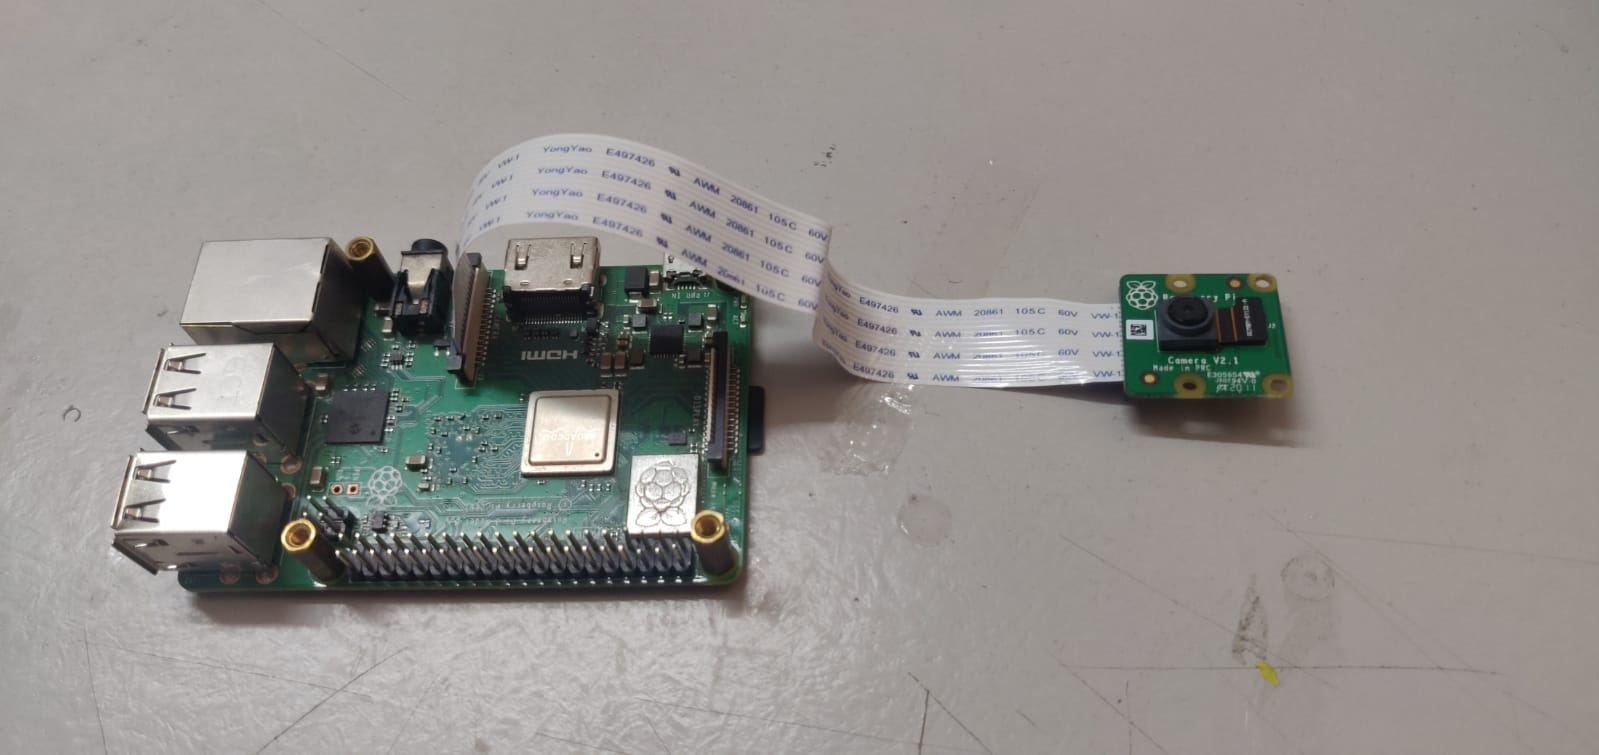
\includegraphics[width=\linewidth]{./figs/hardware/cam.jpeg}
            \endminipage\hfill
            \minipage{0.46\textwidth}
              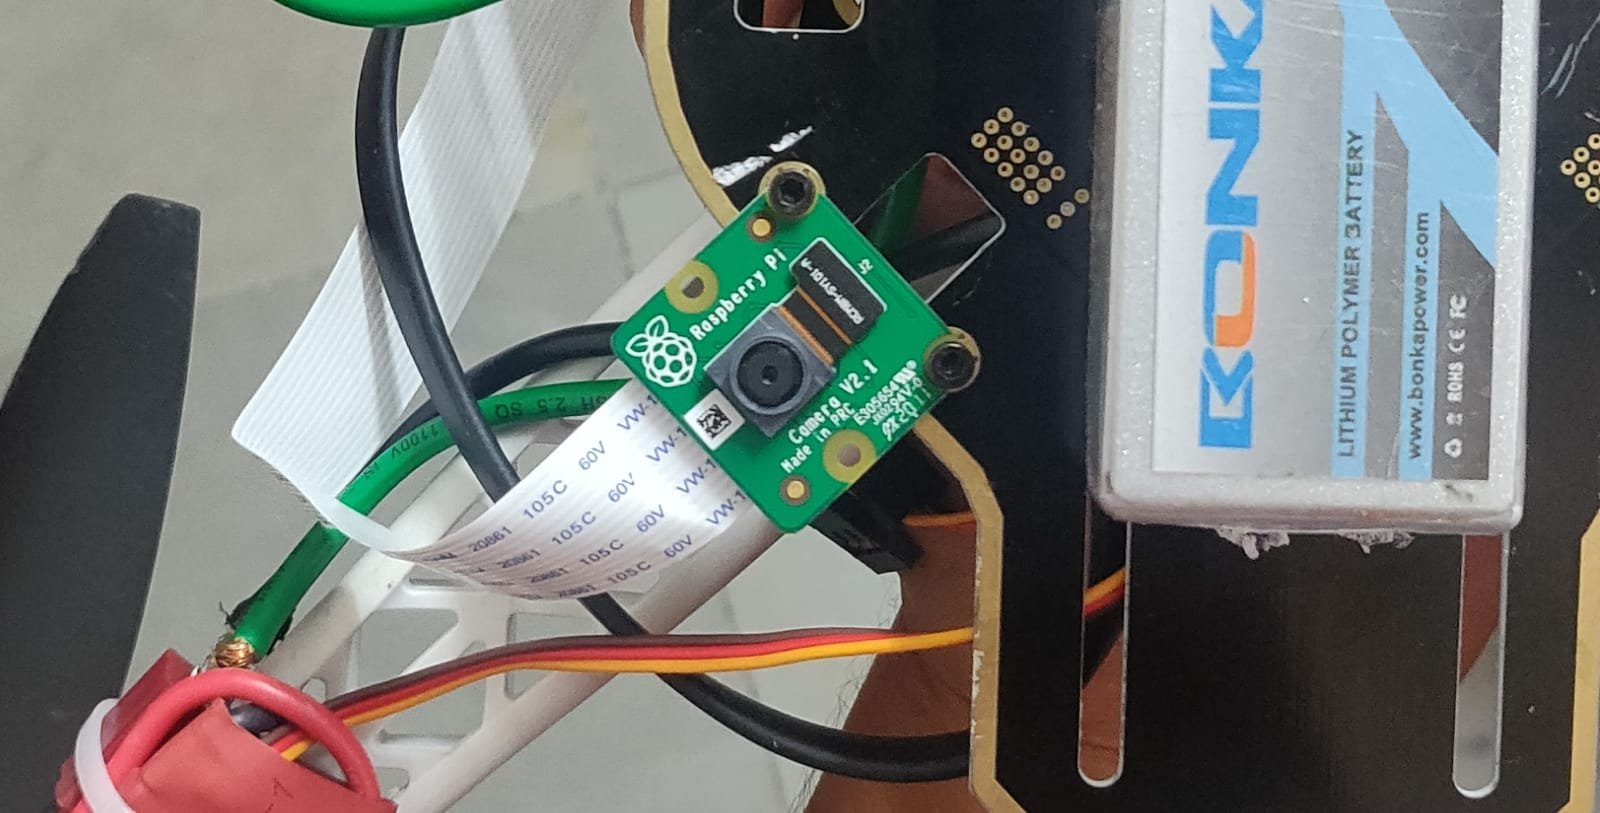
\includegraphics[width=\linewidth]{./figs/hardware/camfixed.jpeg}
            \endminipage
\end{figure}



The intrinsics of the camera must be obtained through a good camera calibration in order for OpenCV computer vision scripts to work. Install VNC viewer on your android device.
Connect the RPi to termux and type the following commands:
\begin{lstlisting}
$ sudo apt-get install realvnc-vnc-server
$ vncserver
\end{lstlisting}
Copy the IP address and port from the output, open the VNC Viewer app and select add network option. Add the IP address and port and connect to the network. The RPi desktop display should be obtained. Open the terminal in this display and type the following commands:
\begin{lstlisting}
$ sudo apt-get install x11-apps
$ xclock
\end{lstlisting}
One should be able to see the clock display pop up on the screen.\\
Camera permissions for RPi:
\begin{lstlisting}
$ sudo raspi-config
\end{lstlisting}
Select Interfacing options, click on "Enabled" for the camera and hit "OK". \\
Now lets begin with calibration:
\begin{lstlisting}
$ git clone https://github.com/neildhami18/video2calibration
$ cd video2calibration
\end{lstlisting}
Print out the pattern.png and glue it to a solid board. Measure the side length of one of the squares in the pattern in millimeters. Place the RPi camera in such a way that the background is white. Type:
\begin{lstlisting}
$ python calibrate.py --mm SideLength --width 640 --height 480
\end{lstlisting}
A video display of the camera feed shall appear on the screen. Bring the pattern printout in front of it and rotate in different orientations. Make sure that the whole board is captured in the camera. After capturing sufficient number of frames, the output data would be stored in the "calibrationFiles" directory.
\\
Figures for reference:
\begin{figure}[!htb]
            \minipage{0.32\textwidth}
              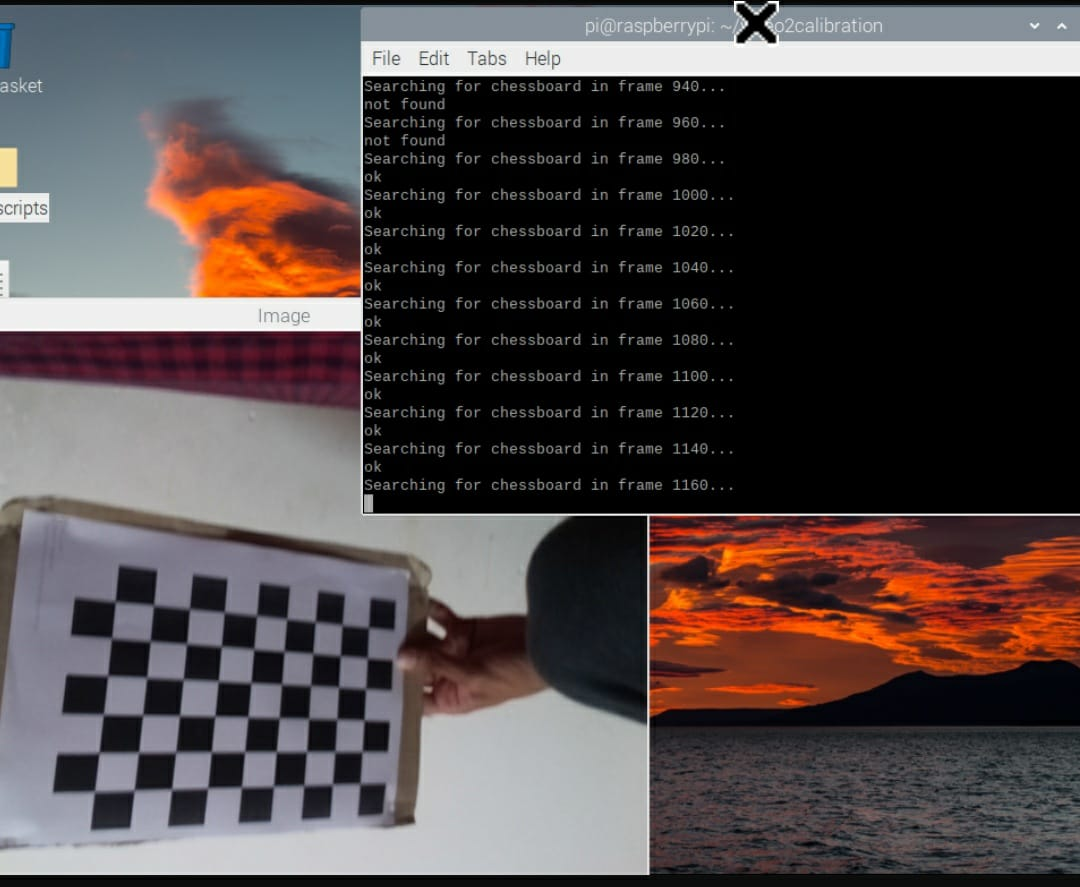
\includegraphics[width=\linewidth]{./figs/images/img1.jpeg}
            \endminipage\hfill
            \minipage{0.32\textwidth}
              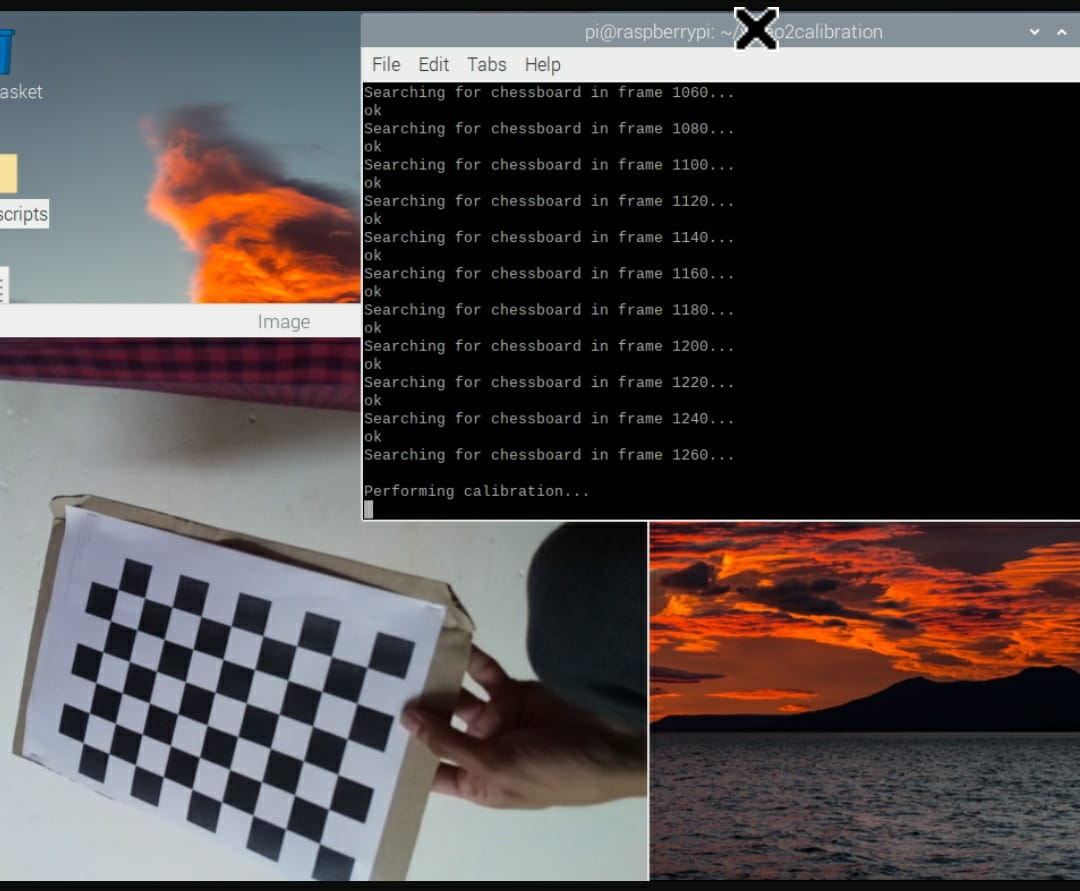
\includegraphics[width=\linewidth]{./figs/images/img2.jpeg}
            \endminipage\hfill
            \minipage{0.33\textwidth}%
              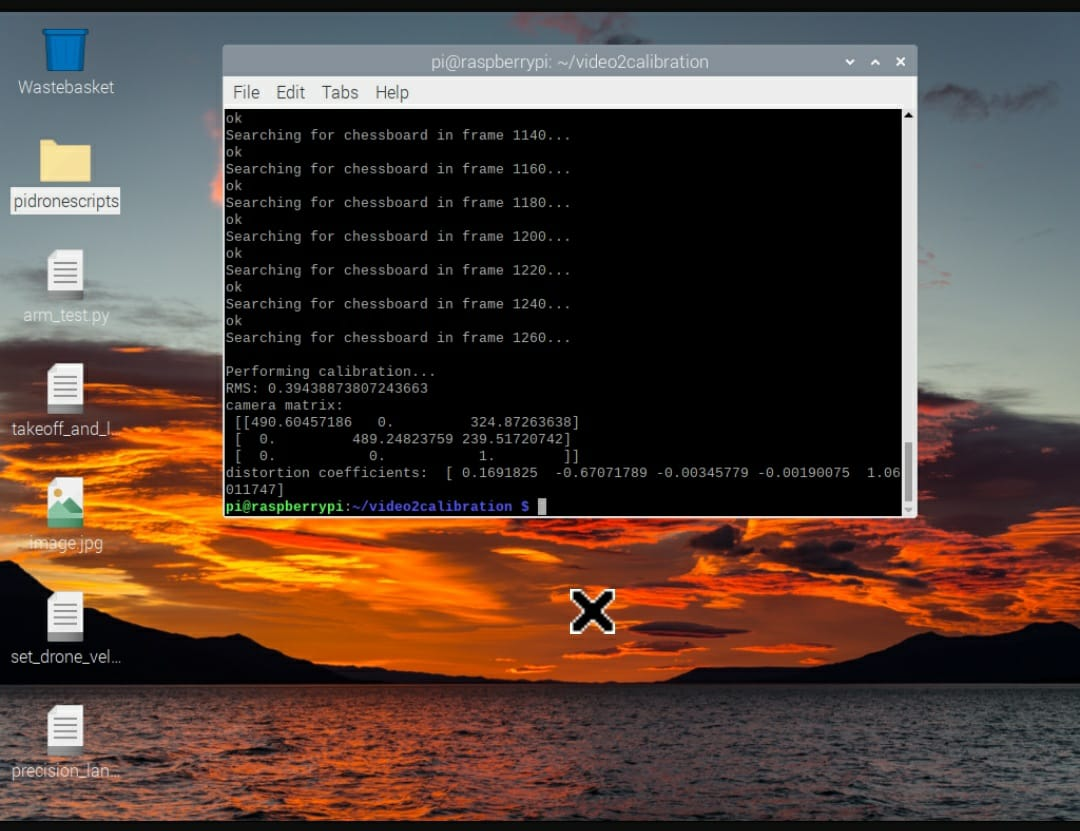
\includegraphics[width=\linewidth]{./figs/images/img3.jpeg}
            \endminipage
\end{figure}

\section{Testing}

\subsection{Installing packages}
Install the following packages
\begin{lstlisting}[language=bash]
    $ pip uninstall opencv-python
    $ pip install opencv-contrib-python
    $ pip install -U numpy 
    $ sudo apt-get install libcblas-dev libhdf5-dev libhdf5-serial-dev libatlas-base-dev libjasper-dev libqtgui4 libqt4-test
\end{lstlisting}
 
\subsection{Aruco Detection}
Print the aruco marker (id=72) with a side length of around 17.5cm and glue it to a solid board. Write a python script to detect and confirm the id of the aruco marker. 
\\
The python script is available at the repository:
\begin{lstlisting}
https://github.com/neildhami18/IITH_Academics/DroneIDP-2022/Manual-3/codes/aruco_tester.py
\end{lstlisting}

Figures for reference:
\begin{figure}[!htb]
            \minipage{0.48\textwidth}
              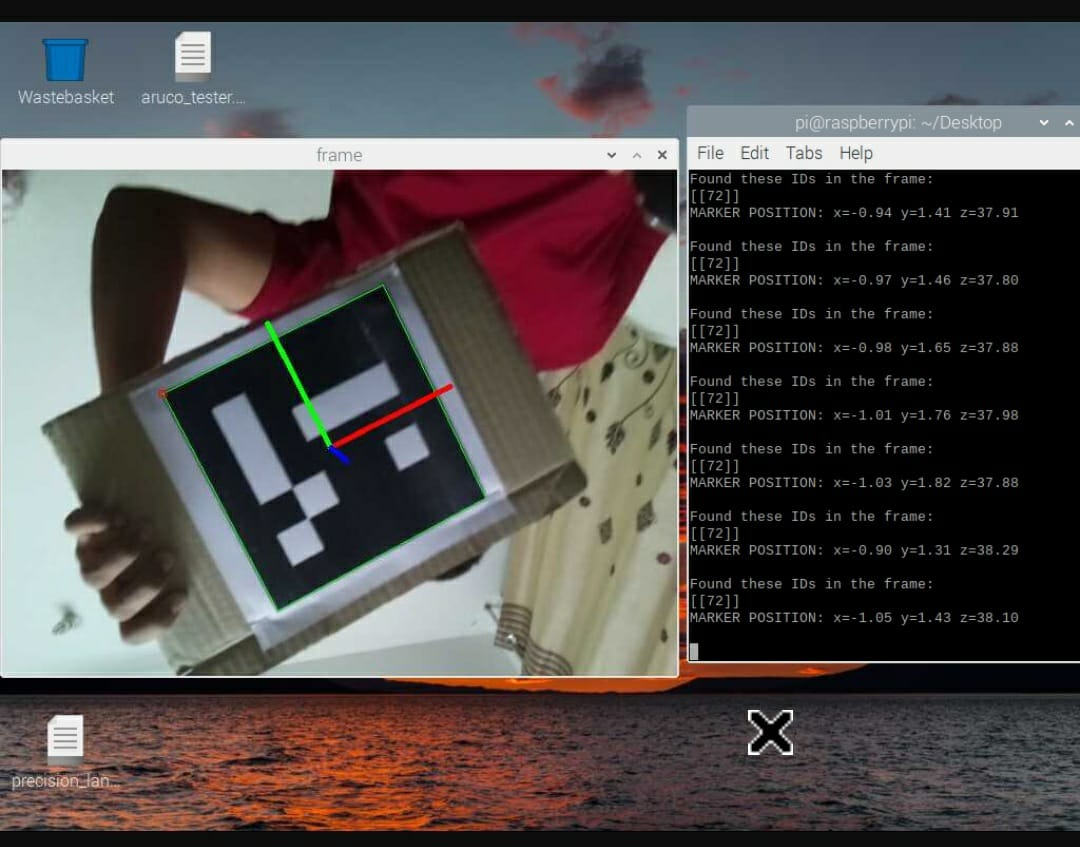
\includegraphics[width=\linewidth]{./figs/images/aruco1.jpeg}
            \endminipage\hfill
            \minipage{0.48\textwidth}
              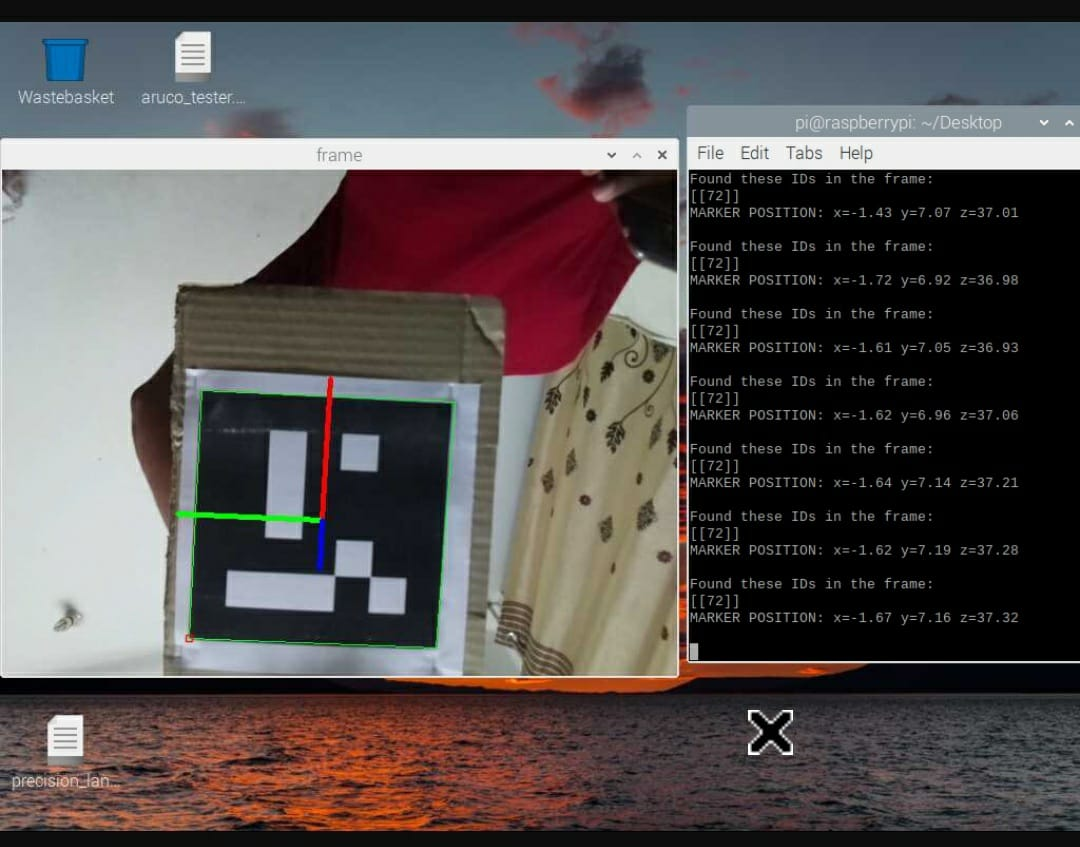
\includegraphics[width=\linewidth]{./figs/images/aruco2.jpeg}
            \endminipage
\end{figure}

Now that our RPi camera is able to successfully detect the aruco marker, lets proceed to the precision landing experiment.


\section{Precision Landing Experiment}
Place the Aruco markers of ids 72 (side=17.5cm) and 129 (side=25cm) arbitrarily in an open ground. Obtain the latitudinal and longitudinal coordinates at the aruco markers' position using Google Maps. Write a python script to fly the drone from another point to the given coordinates and land on the aruco markers. The landing function could be defines as:
\begin{lstlisting}[language=Python]
def lander():
    global first_run,notfound_count,found_count,marker_size,start_time
    if first_run==0:
        print("First run of lander!!")
        first_run=1
        start_time=time.time()

    id_found=0
    frame = cap.read()
    frame = cv2.resize(frame,(horizontal_res,vertical_res))
    frame_np = np.array(frame)
    gray_img = cv2.cvtColor(frame_np,cv2.COLOR_BGR2GRAY)
    ids=''
    corners, ids, rejected = aruco.detectMarkers(image=gray_img,dictionary=aruco_dict,parameters=parameters)
    if vehicle.mode!='LAND':
        vehicle.mode=VehicleMode("LAND")
        while vehicle.mode!='LAND':
            print('WAITING FOR DRONE TO ENTER LAND MODE')
            time.sleep(1)

    counter=0
    corners_np = np.asarray(corners)

    id_to_find=0
    marker_height=0
    marker_size=0
    altitude = vehicle.location.global_relative_frame.alt ##Use vehicle.rangefinder.distance if rangefinder data desired instead

    if altitude > marker_heights[1]:
        id_to_find=ids_to_find[0]
        marker_height=marker_heights[0]
        marker_size=marker_sizes[0]
    elif altitude < marker_heights[1]:
        id_to_find=ids_to_find[1]
        marker_height=marker_heights[1]
        marker_size=marker_sizes[1]

    print("Marker "+str(id_to_find)+"at "+str(marker_size)+" cms.")

    try:
        if ids is not None:
            for id in ids:
                if id == id_to_find:
                    corners_single = [corners[counter]]
                    corners_single_np = np.asarray(corners_single)
                    ret = aruco.estimatePoseSingleMarkers(corners_single,marker_size,cameraMatrix=cameraMatrix,distCoeffs=cameraDistortion)
                    (rvec, tvec) = (ret[0][0, 0, :], ret[1][0, 0, :])
                    x = '{:.2f}'.format(tvec[0])
                    y = '{:.2f}'.format(tvec[1])
                    z = '{:.2f}'.format(tvec[2])

                    y_sum = 0
                    x_sum = 0

                    x_sum = corners_single_np[0][0][0][0]+ corners_single_np[0][0][1][0]+ corners_single_np[0][0][2][0]+ corners_single_np[0][0][3][0]
                    y_sum = corners_single_np[0][0][0][1]+ corners_single_np[0][0][1][1]+ corners_single_np[0][0][2][1]+ corners_single_np[0][0][3][1]

                    x_avg = x_sum*.25
                    y_avg = y_sum*.25
            
                    x_ang = (x_avg - horizontal_res*.5)*(horizontal_fov/horizontal_res)
                    y_ang = (y_avg - vertical_res*.5)*(vertical_fov/vertical_res)
            
                    if vehicle.mode!='LAND':
                        vehicle.mode = VehicleMode('LAND')
                        while vehicle.mode!='LAND':
                            time.sleep(1)
                        print("------------------------")
                        print("Vehicle now in LAND mode")
                        print("------------------------")
                        send_land_message(x_ang,y_ang)
                    else:
                        send_land_message(x_ang,y_ang)
                        pass
                    print("X CENTER PIXEL: "+str(x_avg)+" Y CENTER PIXEL: "+str(y_avg))
                    print("FOUND COUNT: "+str(found_count)+" NOTFOUND COUNT: "+str(notfound_count))
                    print("MARKER POSITION: x=" +x+" y= "+y+" z="+z)
                    found_count=found_count+1
                    id_found=1
                    print("")
                counter=counter+1
            if id_found==0:
                notfound_count=notfound_count+1
        else:
            notfound_count=notfound_count+1
    except Exception as e:
        print('Target likely not found. Error: '+str(e))
        notfound_count=notfound_count+1
    

\end{lstlisting}



\end{document}

